\documentclass{article}
\setlength{\parskip}{0pt} % esp. entre parrafos
\setlength{\parindent}{20pt} % esp. al inicio de un parrafo
\usepackage{amsmath} % mates
\usepackage{listings}
\usepackage{xcolor}
\usepackage[sort&compress,numbers]{natbib} % referencias
\usepackage{url} % que las URLs se vean lindos
\usepackage[top=10mm,left=20mm,right=20mm,bottom=25mm]{geometry} % \textbf{\textbf{}}margenes
\usepackage{hyperref} % ligas de URLs
\usepackage{graphicx} % poner figuras
\usepackage{caption}
\usepackage{subcaption}
\usepackage[spanish]{babel} % otros idiomas
\hypersetup{
    colorlinks=true,
    linkcolor=blue,
    filecolor=blue,      
    urlcolor=blue,
}
\renewcommand{\lstlistingname}{Código}
\definecolor{codeblack}{rgb}{0,0.6,0}
\definecolor{codegray}{rgb}{0.5,0.5,0.5}
\definecolor{codepurple}{rgb}{0.58,0,0.82}
\definecolor{backcolour}{rgb}{0.95,0.95,0.92}
\lstdefinestyle{mystyle}{
    backgroundcolor=\color{backcolour},   
    commentstyle=\color{codeblack},
    keywordstyle=\color{blue},
    numberstyle=\tiny\color{codegray},
    stringstyle=\color{codeblack},
    basicstyle=\ttfamily\footnotesize,
    breakatwhitespace=false,         
    breaklines=true,                 
    keepspaces=true,                 
    numbers=left,                    
    numbersep=5pt,                  
    showspaces=false,                
    showstringspaces=false,
    showtabs=false,                  
    tabsize=2
}
\lstset{style=mystyle}

\title{"P4" Diagramas de Voronoi}
\author{NESTOR}
\date {Marzo 2022}

\begin{document}

\maketitle

\section{Objetivo}\label{obj}
El objetivo de la práctica consiste en un espacio bidimensional una zona con medidas conocidas que contiene  puntos semilla , representados por sus coordenadas. Lo que se busca es dividir esa zona en regiones llamadas celdas de Voronoi de tal forma que todos los puntos que pertenecen a la región que estén más cerca de esa semilla que a cualquier otra.

\section{Desarrollo}\label{des}
Basando el desarrollo en la \href{https://github.com/satuelisa/Simulation/blob/master/VoronoiDiagrams/fracture.py}{codificación} implementado por E. Schaeffer \cite{elisa1} y se encuentra todas las instrucciones en el repositorio \href{https://github.com/NestorZeus/SIMULACION-COMPUTACIONAL-DE-NANOMATERIALES/tree/main/P4}{repositorio} de Nestor en GitHub.\\

Para comenzar se hace primero generar el cuadro de las semillas con las funciones.

\begin{lstlisting}[caption=Función con las semillas, language=Python]
def celda(pos):
   if pos in semillas:
   return semillas.index(pos)
   x, y = pos % n, pos // n
   cercano = None
   menor = n * sqrt(2)
   for i in range(k):
   (xs, ys) = semillas[i]
   dx, dy = x - xs, y - ys
   dist = sqrt(dx**2 + dy**2)
   if dist < menor:
   cercano, menor = i, dist
return cercano
\end{lstlisting}

Posteriormente al tener las celdas se crea generar el cuadro con las funciones. Lo siguiente es definir en una función para las semillas y las \href{https://satuelisa.github.io/simulation/p3.html}{grietas} implementados por E. Schaeffer, como se muestra a continuación en el código \ref{codigo2}.

\begin{lstlisting}[caption=Semillas para encontrar grietas, label=codigo2, language=Python]
def inicio():
    direccion = randint(0, 3)
    if direccion == 0: # vertical abajo -> arriba
        return (0, randint(0, n - 1))
    elif direccion == 1: # izq. -> der
        return (randint(0, n - 1), 0)
    elif direccion == 2: # der. -> izq.
        return (randint(0, n - 1), n - 1)
    else:
        return (n - 1, randint(0, n - 1))

 
def propaga(replica,rupturas):
    grieta = voronoi.copy()
    for f in range(rupturas):
        prob, dificil = 0.9, 0.8
        #grieta = voronoi.copy()
        g = grieta.load()
        (x, y) = inicio()
        largo = 0
        cnt=0
        if f == 0:
            color=(0,0,0)# grieta color negro
        if f == 1:
            color = (0, 0, 255)# color azul de grieta para el segundo ciclo
        while True:
            g[x, y] = color
            largo += 1
            frontera, interior = [], []
\end{lstlisting}

Para saber el programa de como se genera el cuadro que se llama las funciones y se pueda generar, \href{https://satuelisa.github.io/simulation/p3.html}{grietas} implementados por E. Schaeffer, se muestra a continuación en el código \ref{codigo3}.

\begin{lstlisting}[caption=Ejecuci\'on de c\'odigos, label=codigo3, language=Python]
for k in 5, 80, 250:
   ciclos=ciclos+1
   print("########## semillas",k,"##############")
   for s in range(k):
    while True:
    x, y = randint(0, n - 1), randint(0, n - 1)
    if (x, y) not in semillas:
    semillas.append((x, y))
    break
    
    celdas = [celda(i) for i in range(n * n)]
    voronoi = Image.new('RGB', (n, n))
    vor = voronoi.load()
    c = sns.color_palette("Set3", k).as_hex()
    for i in range(n * n):
    vor[i % n, i // n] = ImageColor.getrgb(c[celdas.pop(0)])
    limite, vecinos = 1, []

\end{lstlisting}

Se realiza para saber las réplicas y en la función de la grieta, se agrega aparte de que haga los ciclos de cincuenta veces, se agrega variables que se conoce como: rupturas.  \texttt a continuación se muestra el siguiente código.

\begin{lstlisting}[caption=Rupturas, label=codigo5, language=Python]
rupturas=2# cantidad de grietas
        contacto=[]
        for r in range(300): # replicas
            atraveso = propaga(r,rupturas)
            #print("Por replica:",r, "resultado:",atraveso)
        print("cuantos atravesaron",len(atraveso))
        if ciclos == 1:
            prob["min_sem"].append(((len(atraveso))/300)*100)
        if ciclos == 2:
            prob["med_sem"].append(((len(atraveso))/300)*100)
        if ciclos == 3:
            prob["max_sem"].append(((len(atraveso))/300)*100)
    print("final de probabilidades",prob)
\end{lstlisting}

\section{Resultados}\label{res}

A continuación se muestra las semillas y las grietas, en la figura 1. Donde se da a demostrar que las grietas no se tocan figura 1a, y otro donde las grietas se tocan figura 1b. En la figura 2 se muestra las gietas de las semillas de mayor valor 2a y 2b. Posteriormente, en la figura 3 se muestran el porcentaje de las probabilidades que se calcularon de las grietas de las semillas con las dimensiones. Y finalmente una analisis de los datos multivariados en la figura 4.

\begin{figure}
     \centering
     \begin{subfigure}[b]{0.40\textwidth}
         \centering
         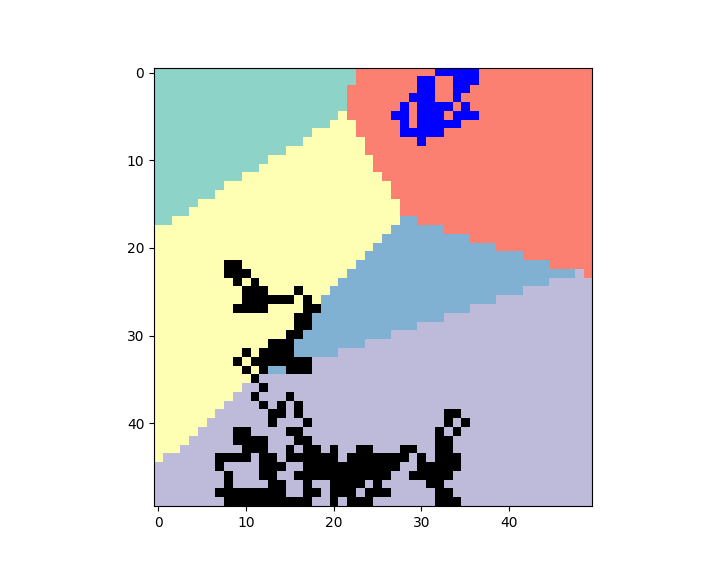
\includegraphics[width=\textwidth]{Figure_1.png}
         \caption{Las grietas no se tocan.}
         \label{fig:notocan}
     \end{subfigure}
     \begin{subfigure}[b]{0.45\textwidth}
         \centering
         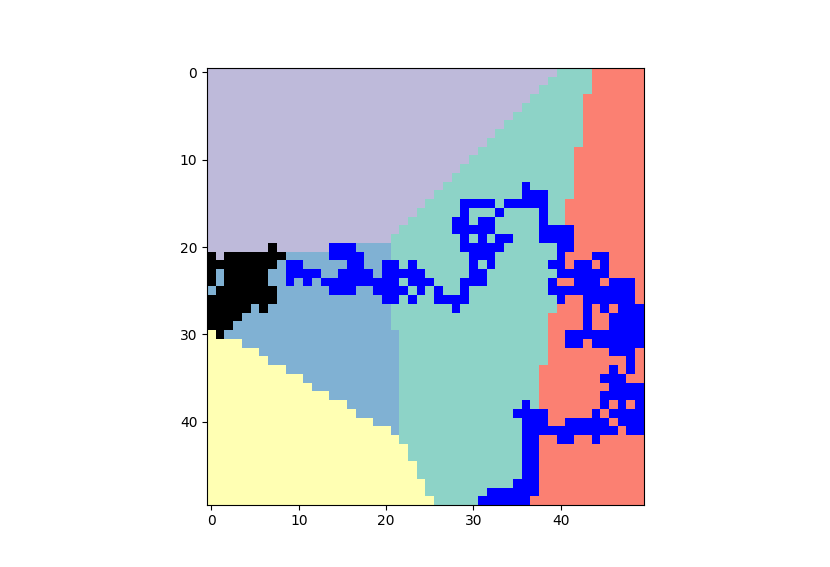
\includegraphics[width=\textwidth]{Figure_2.png}
         \caption{Las grietas se tocan.}
         \label{fig:tocan}
     \end{subfigure}
     \caption{Grietas.}
     \label{grietas}
     
     \centering
     \begin{subfigure}[b]{0.45\textwidth}
         \centering
         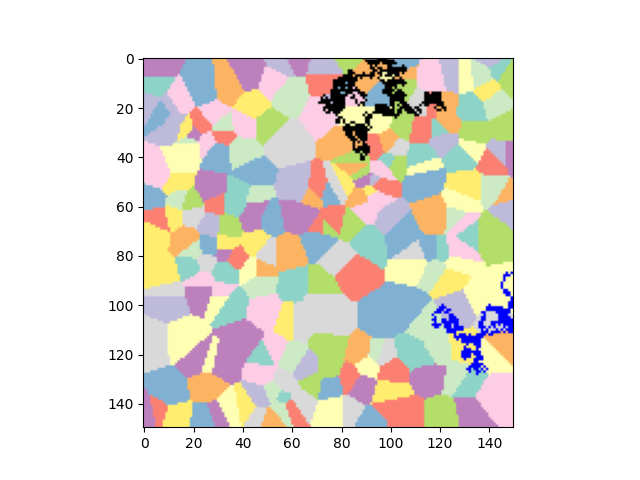
\includegraphics[width=\textwidth]{Figure_3.png}
         \caption{Las grietas no se tocan.}
         \label{fig:notocan}
     \end{subfigure}
     \begin{subfigure}[b]{0.45\textwidth}
         \centering
         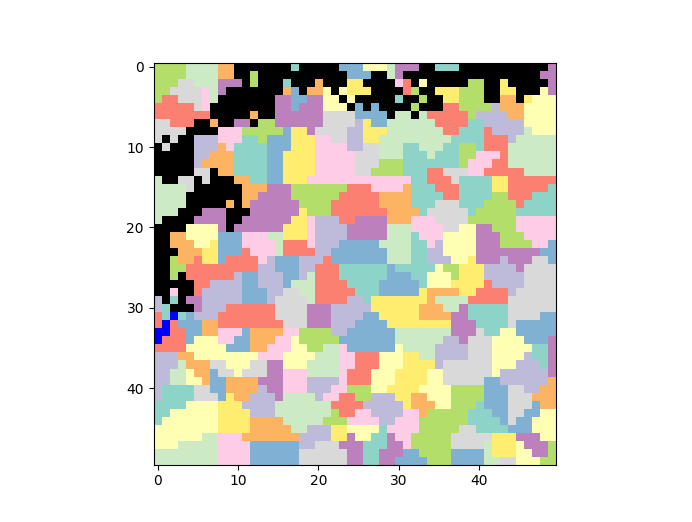
\includegraphics[width=\textwidth]{Figure_4.png}
         \caption{Las grietas se tocan.}
         \label{fig:tocan}
     \end{subfigure}
     \caption{Semillas de grietas de mayor valor.}
     \label{grietas}
      

\end{figure}

\newpage
 \begin{subfigure}{1.1\textwidth}
         \centering
         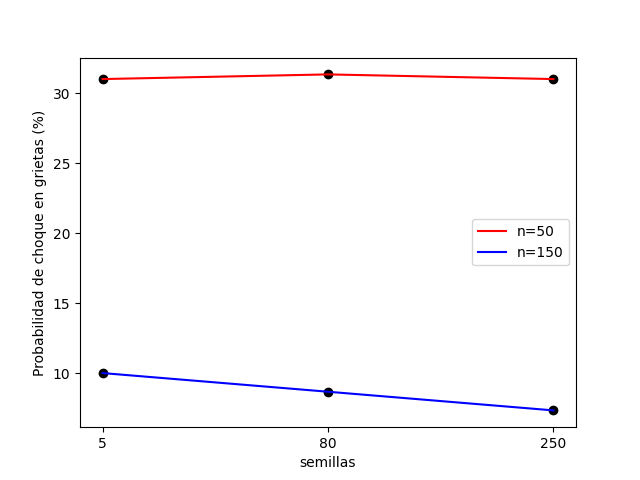
\includegraphics[width=\textwidth]{Figure_5.png}
         \caption{Las grietas se tocan.}
         \label{fig:tocan}
     \end{subfigure}
     \caption{Semillas de grietas de mayor valor.}
     \label{grietas}
\end{figure}
     
Figura 3: Probabilidad de las grietas

\newpage

\subsection{Radar Chart}\label{con}
Una Gráfica de Radar, también conocida como un diagrama de araña, es una herramienta muy útil para mostrar visualmente los gaps entre el estado actual y el estado ideal. \cite{Matpltlib}.
A continuación se presenta visualmente los gaps existentes entre el estado actual y el estado ideal.
  
    \begin{subfigure}{1.09\textwidth}
         \centering
         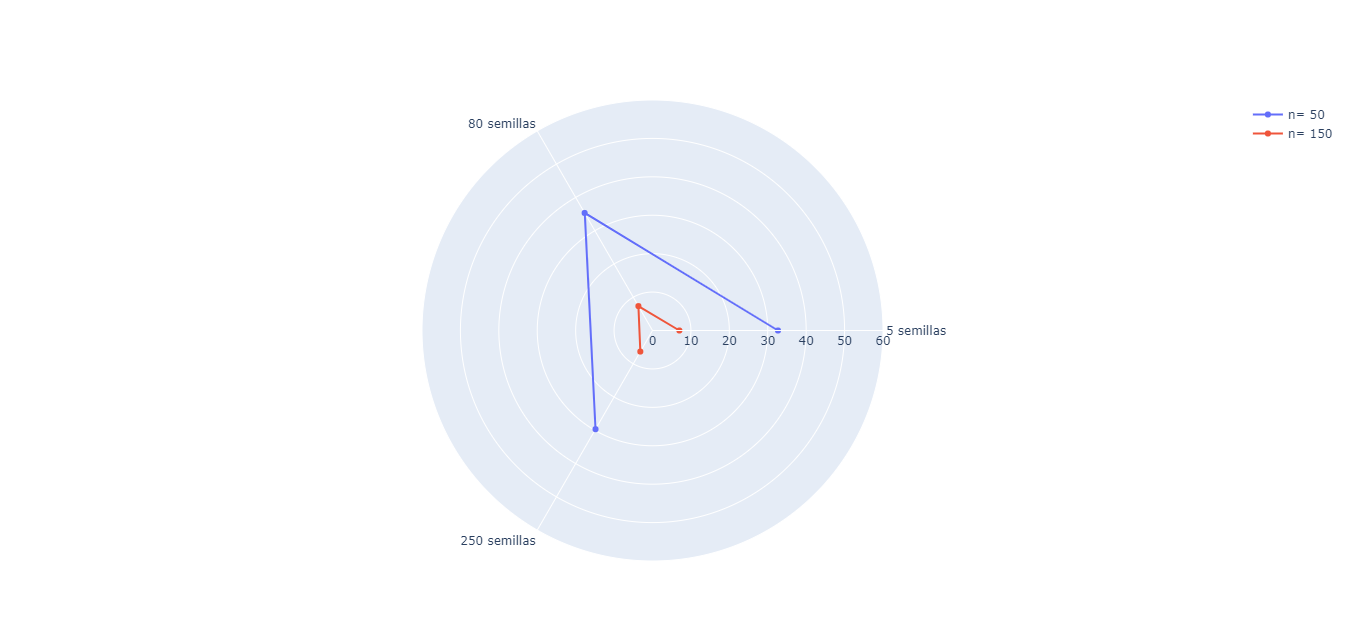
\includegraphics[width=\textwidth]{Figure_6.png}
         \caption{Analisis}
         \label{fig:tocan}
     \end{subfigure}
     \caption{Semillas de grietas de mayor valor.}
     \label{grietas}
     Figura 4: Analisis de los datos multivariados


\section{Conclusiones}\label{con}
Se concluye que las fronteras va aumentando con respecto a la cantidad de semillas, ya que las grietas no se aminoran. Sin embargo en la gráfica de radar chart nos muestra como se comporta las semillas dando valores multivariados.


\section{Reto 1}\label{con}
En este reto consiste en crecer las celdas dinámicamente alrededor de semillas de tal forma que las semillas aparecen al azar en distintas iteraciones y crecen con una tasa exponencialmente distribuida (variable entre núcleos pero constante para un núcleo específico) hasta toparse con las demás celdas, así como se muestra en la animación. Examina los cambios producidos en el fenómeno de propagación de grietas que esta nueva forma de crear las celdas provoca, ya que las semillas resultan en celdas de tamaños distintos según su edad y su tasa, además del efecto de la posición relativa a las demas semillas \cite{elisa1}.

Para esto se crea una función para la visualización y creación de las semillas de como van creciendo ya que la práctica es lo mismo, este reto consiste si las grietas chocan solo que se modifican la creación de las semillas como se muestra en las siguientes instrucciones: 


\begin{lstlisting}[caption=Función con las semillas, language=Python]
def union(seeds,im,incr):
  for a in range(len(seeds)):
    x=seeds[a][0]
    y=seeds[a][1]
    r = incr[a]
    color=im.getpixel((x, y))
    img=im.copy()
    image = img
    draw = ImageDraw.Draw(image)
    draw.ellipse((x-r, y-r, x+r, y+r), fill=color)
    for Y in range(n):
\end{lstlisting}
               
Luego creamos la posición y color de las semillas como se mjuestra en la siguiente instrucción:

\begin{lstlisting}[caption=Posición y Color de las semillas, language=Python]
for s in range(k):
            while True:
                x, y = randint(0, n - 1), randint(0, n - 1)
                if (x, y) not in semillas:
                    semillas.append((x, y))
                    break
        col=[]
        for dato in paleta:
            col.append([(int(i * 255)) for i in dato])
\end{lstlisting}

Para saber el comportamiento de las semmillas y el crecimiento, se muestra en la siguiente instrucción: 

\begin{lstlisting}[caption=Comportamiento y Crecimiento de las semillas, language=Python]
for i in range(len(semillas)):
  voronoi.putpixel(semillas[i],(tuple(col[i])))
    #plt.imshow(voronoi)###### IMPRIMIR
    #plt.show()
    #vo=voronoi.copy()
    #visual = vo.resize((10 * n,10 * n))
    #visual.save("ciclo_0_ini.png")
    p=0.4
    aumento=[]
    semi=[]
    for s in range(n):
    #fondo=[]
    #print("######## ciclo:",s)
    if s == 0:
      semi.append(semillas[0])
      semillas.pop(s)
      aumento.append(0)
\end{lstlisting}

Para obtener los resultados se muestra para las semillas que se crearon, fueron creciendo hasta que se cristalizó con el aumento de más semillas como se muestra a continuación:

\begin{lstlisting}[caption=Obtención del resultado comportamiento del crecimiento de las semillas, language=Python]
if s != 0 and ((random.uniform(0, 1)) > p) and len(semillas)>0:
                rnd=random.choice(semillas)
                semi.append(rnd)
                semillas.remove(rnd)
                aumento.append(0)
            aumento=[s+1 for s in aumento]
            voronoi= union(semi,voronoi,aumento)
            #[[fondo.append(voronoi.getpixel((x,y))) for x in range(5)]for y in range(5)]
            #vis=voronoi.copy()
            #visual = vis.resize((10 * n,10 * n))
            #visual.save("ciclo_{:d}.png".format(s))
            #plt.imshow(voronoi)
            #plt.show()
        #plt.imshow(voronoi)####### IMPRIMIR
        #plt.show()###############
\end{lstlisting}


\section{Reto 1 resultados}\label{con}
Con el aumento de más semillas se cristalizó y se analizó lo mismo del comportamiento de las grietas. Se encuentra todos los resultados y gifs en el repositorio \href{https://github.com/NestorZeus/SIMULACION-COMPUTACIONAL-DE-NANOMATERIALES/tree/main/P4}{repositorio} de Nestor en GitHub.\\

\begin{figura_7}
\end{figura_7}
    \centering
    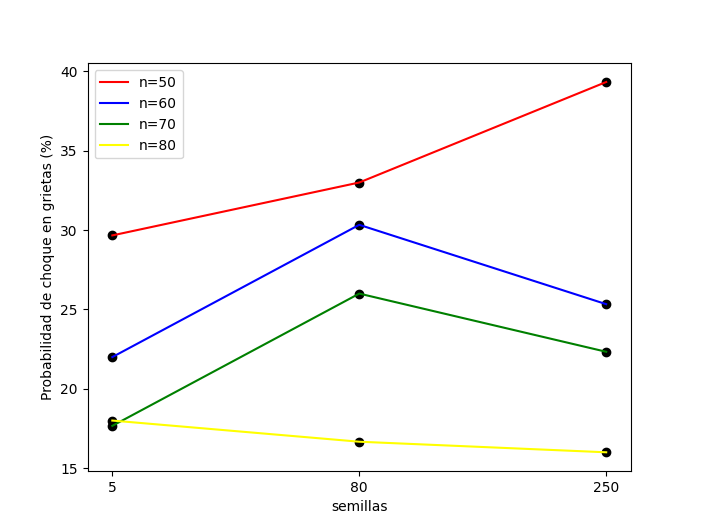
\includegraphics[width=215mm]{Figura_7.png}
    \caption{Figura 1: Prueba de Algoritmo}
    \label{figura_7}
\end{figure}


\begin{figure}
     \centering
     \begin{subfigure}[b]{0.40\textwidth}
         \centering
         
\includegraphics[width=\textwidth]{ciclo_11.png}
         \caption{Las fronteras no se tocan.}
         \label{fig:notocan}
     \end{subfigure}
     \begin{subfigure}[b]{0.40\textwidth}
         \centering
         
\includegraphics[width=\textwidth]{ciclo_33.png}
         \caption{Las fronteras se tocan.}
         \label{fig:tocan}
     \end{subfigure}
     \caption{Intervalo de 10 Semillas de las Grietas}
      \label{semilla}
\end{figure}

\begin{figure}
     \centering
     \begin{subfigure}[b]{0.40\textwidth}
         \centering
         \includegraphics[width=\textwidth]{ciclo_12.png}
         \caption{Las fronteras no se tocan.}
         \label{fig:notocan}
     \end{subfigure}
     \begin{subfigure}[b]{0.40\textwidth}
         \centering
         
\includegraphics[width=\textwidth]{ciclo_36.png}
         \caption{Las fronteras se tocan.}
         \label{fig:tocan}
     \end{subfigure}
     \caption{Intervalo de 80 Semillas de las Grietas}
      \label{semilla}
\end{figure}

\begin{figure}
     \centering
     \begin{subfigure}[b]{0.40\textwidth}
         \centering
         
\includegraphics[width=\textwidth]{ciclo_5.png}
         \caption{Las fronteras no se tocan.}
         \label{fig:notocan}
     \end{subfigure}
     \begin{subfigure}[b]{0.40\textwidth}
         \centering
         
\includegraphics[width=\textwidth]{ciclo_30.png}
         \caption{Las fronteras se tocan.}
         \label{fig:tocan}
     \end{subfigure}
     \caption{Intervalo de 100 Semillas de las Grietas}
      \label{semilla}
\end{figure}
\newpage

\bibliographystyle{plain}
\bibliography{simulacion}

\cite{Matpltlib}
\end{document}
